\documentclass[10pt]{article}
\usepackage[english]{babel}
\usepackage[utf8]{inputenc}
\usepackage{amsmath}
\usepackage{listings}
\usepackage{tikz}

\title{\vspace{-5.0cm}LaTeX tikz EXAMPLES}
\author{\vspace{-0.1cm}Jeff DeCola}
\date{\vspace{-1.0cm}}

\setlength{\parindent}{0em} %Paragraph Indent
\setlength{\parskip}{1em} %Paragraph Spacing

\begin{document}
\maketitle

\textbf{This will draw a circle,}

\begin{lstlisting}
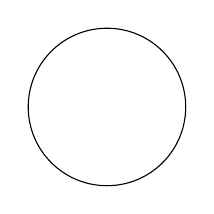
\begin{tikzpicture}
    \draw (2,2) circle (1cm);
\end{tikzpicture}
\end{lstlisting}

\begin{center}
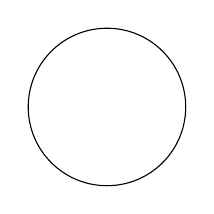
\begin{tikzpicture}
    \draw (2,2) circle (1cm);
\end{tikzpicture}
\end{center}

\textbf{This will draw a blue rectangle,}

\begin{lstlisting}

\begin{tikzpicture}
        \draw [blue] (0,0) rectangle (2,1);
\end{tikzpicture}
\end{lstlisting}

\begin{center}

\begin{tikzpicture}
        \draw [blue] (0,0) rectangle (2,1);
\end{tikzpicture}
\end{center}

\end{document}
